% Fixture: graphics-eps
%
% Purpose: verify per-extension ignore-line patterns for EPS %%CreationDate.
%
% Expected maketex behaviour:
%   - Engine: pdflatex
%   - Passes: 1 (no cross-references, bibliography, or ToC)
%   - Aux tools: none (epstopdf is invoked automatically by the epstopdf package)
%   - Output: main.pdf
%
% EPS files typically contain a %%CreationDate: line that changes on every
% re-export (e.g. from Inkscape or Illustrator).  Without a per-extension
% ignore pattern this would cause endless reruns because the file's hash
% changes even though the graphics content is identical.
%
% The driver must register an ignore regex for the .eps extension that strips
% lines matching /^%%CreationDate:/ before computing the content hash.
% See: Blake3Hasher::setIgnorePattern("eps", "^%%CreationDate: ")
%
% pdflatex cannot include EPS directly; the epstopdf package transparently
% converts figure.eps → figure-eps-converted-to.pdf via shell-escape or a
% restricted \write18 call, then includes the PDF.

\documentclass{article}
\usepackage{graphicx}
\usepackage{epstopdf}

\title{EPS Graphics Test}
\author{Test Fixture}
\date{2026-06-07}

\begin{document}

\maketitle

\section{EPS figure}

The figure below is included from an EPS file whose \texttt{\%\%CreationDate:}
header line should be ignored when computing the content hash, to prevent
false reruns when the date changes but the graphics content does not.

\begin{figure}[h]
  \centering
  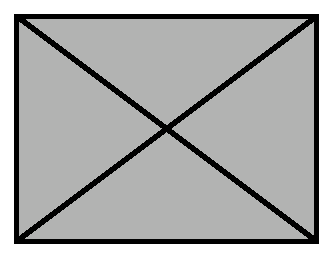
\includegraphics[width=6cm]{figure}
  \caption{A simple PostScript rectangle with a diagonal cross.}
\end{figure}

\end{document}
